%%%%%%%%%%%%%%%%%%%%%%%%%%%%%%%%%%%%%%%%%%%%%%%%%%%%%%%%%%%%%%%%%%%%%%%%%%%%%%%%%%%%%%%%%
% CRAWLAB Poster Submission - ULL E&T Week 2021 
% Andrew Albright
% andrew.albright1@louisiana.edu
% Template Used:
%
% CRAWLAB Poster Template - 03/29/16
% Joshua Vaughan
% joshua.vaughan@louisiana.edu
% http://www.ucs.louisiana.edu/~jev9637/
%
% Originally modified from:
% Jacobs Landscape Poster
% LaTeX Template
% Version 1.1 (14/06/14)
%
% Created by:
% Computational Physics and Biophysics Group, Jacobs University
% https://teamwork.jacobs-university.de:8443/confluence/display/CoPandBiG/LaTeX+Poster
% 
% Further modified by:
% Nathaniel Johnston (nathaniel@njohnston.ca)
%
% This template has been downloaded from:
% http://www.LaTeXTemplates.com
%
% License:
% CC BY-NC-SA 3.0 (http://creativecommons.org/licenses/by-nc-sa/3.0/)
%
%%%%%%%%%%%%%%%%%%%%%%%%%%%%%%%%%%%%%%%%%%%%%%%%%%%%%%%%%%%%%%%%%%%%%%%%%%%%%%%%%%%%%%%%%

%----------------------------------------------------------------------------------------
%	PACKAGES AND OTHER DOCUMENT CONFIGURATIONS
%----------------------------------------------------------------------------------------

\documentclass[final]{beamer}

\usepackage[scale=1.24]{beamerposter} % Use the beamerposter package for laying out the poster

\usetheme{confposter} % Use the confposter theme supplied with this template

% Colors are set in beamerthemeconfposter.sty

%-----------------------------------------------------------
% Define the column widths and overall poster size
% To set effective sepwid, onecolwid and twocolwid values, first choose how many columns you want and how much separation you want between columns
% In this template, the separation width chosen is 0.024 of the paper width and a 4-column layout
% onecolwid should therefore be (1-(# of columns+1)*sepwid)/# of columns e.g. (1-(4+1)*0.024)/4 = 0.22
% Set twocolwid to be (2*onecolwid)+sepwid = 0.464
% Set threecolwid to be (3*onecolwid)+2*sepwid = 0.708

\newlength{\sepwid}
\newlength{\onecolwid}
\newlength{\twocolwid}
\newlength{\threecolwid}
\setlength{\paperwidth}{48in} % A0 width: 46.8in
\setlength{\paperheight}{36in} % A0 height: 33.1in
\setlength{\sepwid}{0.024\paperwidth} % Separation width (white space) between columns
\setlength{\onecolwid}{0.22\paperwidth} % Width of one column
\setlength{\twocolwid}{0.464\paperwidth} % Width of two columns
\setlength{\threecolwid}{0.708\paperwidth} % Width of three columns
\setlength{\topmargin}{-0.5in} % Reduce the top margin size
%-----------------------------------------------------------

\usepackage{graphicx}  % Required for including images
\usepackage[font=small]{caption}
\usepackage{booktabs} % Top and bottom rules for tables

\usepackage{wrapfig}
\usepackage{subfigure}

%----------------------------------------------------------------------------------------
%	TITLE SECTION 
%----------------------------------------------------------------------------------------

\title{Learning Control Strategies and Design \\ Parameters for Flexible-legged Locomotive Systems} % Poster title

\author{Andrew Albright, Joshua Vaughan} % Author(s)

\institute{andrew.albright1@louisiana.edu} % Institution(s)

%----------------------------------------------------------------------------------------

\begin{document}

\addtobeamertemplate{block end}{}{\vspace*{2ex}} % White space under blocks
\addtobeamertemplate{block alerted end}{}{\vspace*{2ex}} % White space under highlighted (alert) blocks

\setlength{\belowcaptionskip}{2ex} % White space under figures
\setlength\belowdisplayshortskip{2ex} % White space under equations

\begin{frame}[t] % The whole poster is enclosed in one beamer frame

\begin{columns}[t] % The whole poster consists of three major columns, the second of which is split into two columns twice - the [t] option aligns each column's content to the top

\begin{column}{\sepwid}\end{column} % Empty spacer column

\begin{column}{\onecolwid} % The first column

%%----------------------------------------------------------------------------------------
%%	OBJECTIVES
%%----------------------------------------------------------------------------------------
%
%\begin{alertblock}{Objectives}
%
%Lorem ipsum dolor sit amet, consectetur, nunc tellus pulvinar tortor, commodo eleifend risus arcu sed odio:
%\begin{itemize}
%\item Mollis dignissim, magna augue tincidunt dolor, interdum vestibulum urna
%\item Sed aliquet luctus lectus, eget aliquet leo ullamcorper consequat. Vivamus eros sem, iaculis ut euismod non, sollicitudin vel orci.
%\item Nascetur ridiculus mus.  
%\item Euismod non erat. Nam ultricies pellentesque nunc, ultrices volutpat nisl ultrices a.
%\end{itemize}
%
%\end{alertblock}

%----------------------------------------------------------------------------------------
%	INTRODUCTION
%----------------------------------------------------------------------------------------

\begin{block}{Flexible Robotics}
%
\begin{wrapfigure}{l}{0.5\textwidth}
    \captionsetup{justification=centering, labelformat=simple}
    \begin{center}
        \vspace{-0.25 in}
        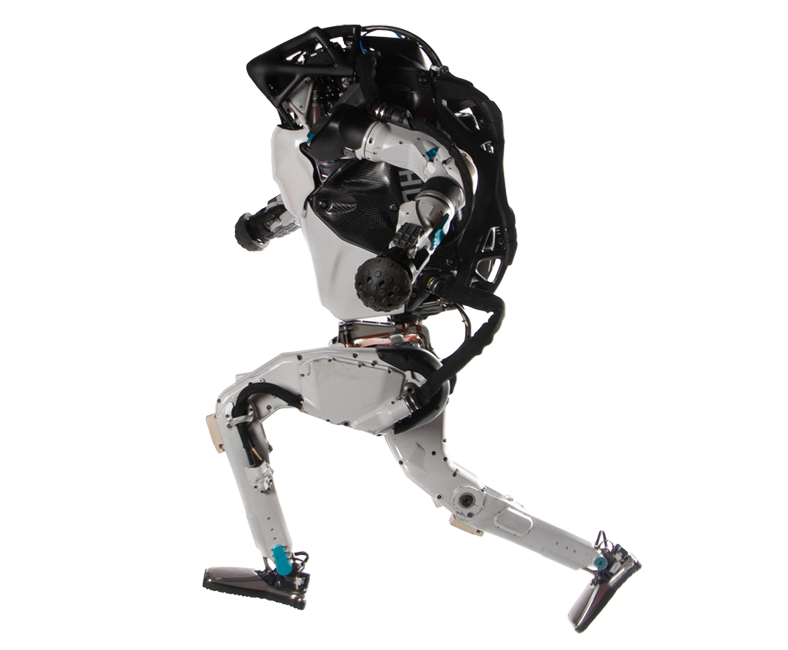
\includegraphics[width=0.46\textwidth]{figures/atlas.png}
        \caption{\:Boston Dynamics Atlas Robot \cite{Atlas}}
        % \vspace{-0.35 in}
        \label{fig:Boston Dynamics Atlas}
    \end{center}
    \captionsetup{justification=centering, labelformat=simple}
    \begin{center}
        \vspace{-0.25 in}
        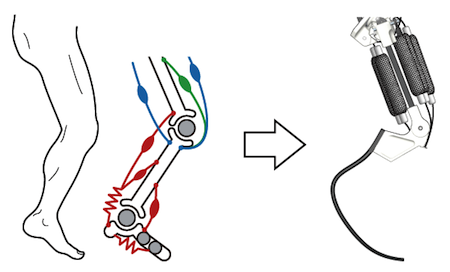
\includegraphics[width=0.46\textwidth]{figures/flexible_leg.png}
        \caption{\:Athlete Robot \cite{Athlete}}
        \vspace{-0.35 in}
        \label{fig:Athlete Robot}
    \end{center}
\end{wrapfigure}
%
% %
% \begin{wrapfigure}{l}{0.5\textwidth}
%     \captionsetup{justification=centering, labelformat=simple}
%     \begin{center}
%         \vspace{-0.25 in}
%         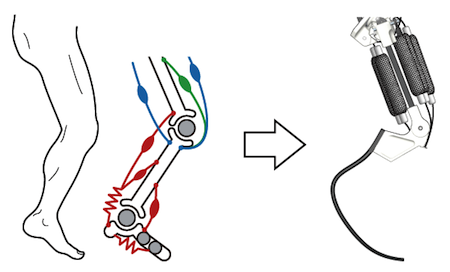
\includegraphics[width=0.46\textwidth]{figures/flexible_leg.png}
%         \caption{\:Athlete Robot \cite{Athlete}}
%         \vspace{-0.35 in}
%         \label{fig:Athlete Robot}
%     \end{center}
% \end{wrapfigure}
% %

Legged systems, like the robot seen in Figure 1, have many advantages compared to their wheeled counterparts. For example, if designed properly, they can more easily navigate uneven and unstable terrain. However, there are disadvantages as well, including dramatically less energy-efficient locomotion. In an effort to mitigate this disadvantage, research has been conducted that shows using flexible components within legged systems, like the ones seen in Figure 2, not only increases their efficiency but also their performance \cite{Sugiyama2004}. However, nonlinear models and controllers for flexible systems are difficult to develop using traditional methods. 

%
%\begin{figure}
%\begin{center}
%
\includegraphics[width = 0.5\columnwidth]{figures/placeholder}
%\caption{Descriptive Caption}
%\label{fig:figure_label}
%\end{center}
%\vspace{-0.2in}
%\end{figure}
%%
\end{block}
%------------------------------------------------



%----------------------------------------------------------------------------------------
%	BACKGROUND Theoretical Knoweldge
%----------------------------------------------------------------------------------------

\begin{block}{Reinforcement Learning}
%
\begin{wrapfigure}{r}{0.55\textwidth}
    \captionsetup{justification=centering, labelformat=simple}
    \begin{center}
        \vspace{-0.25 in}
        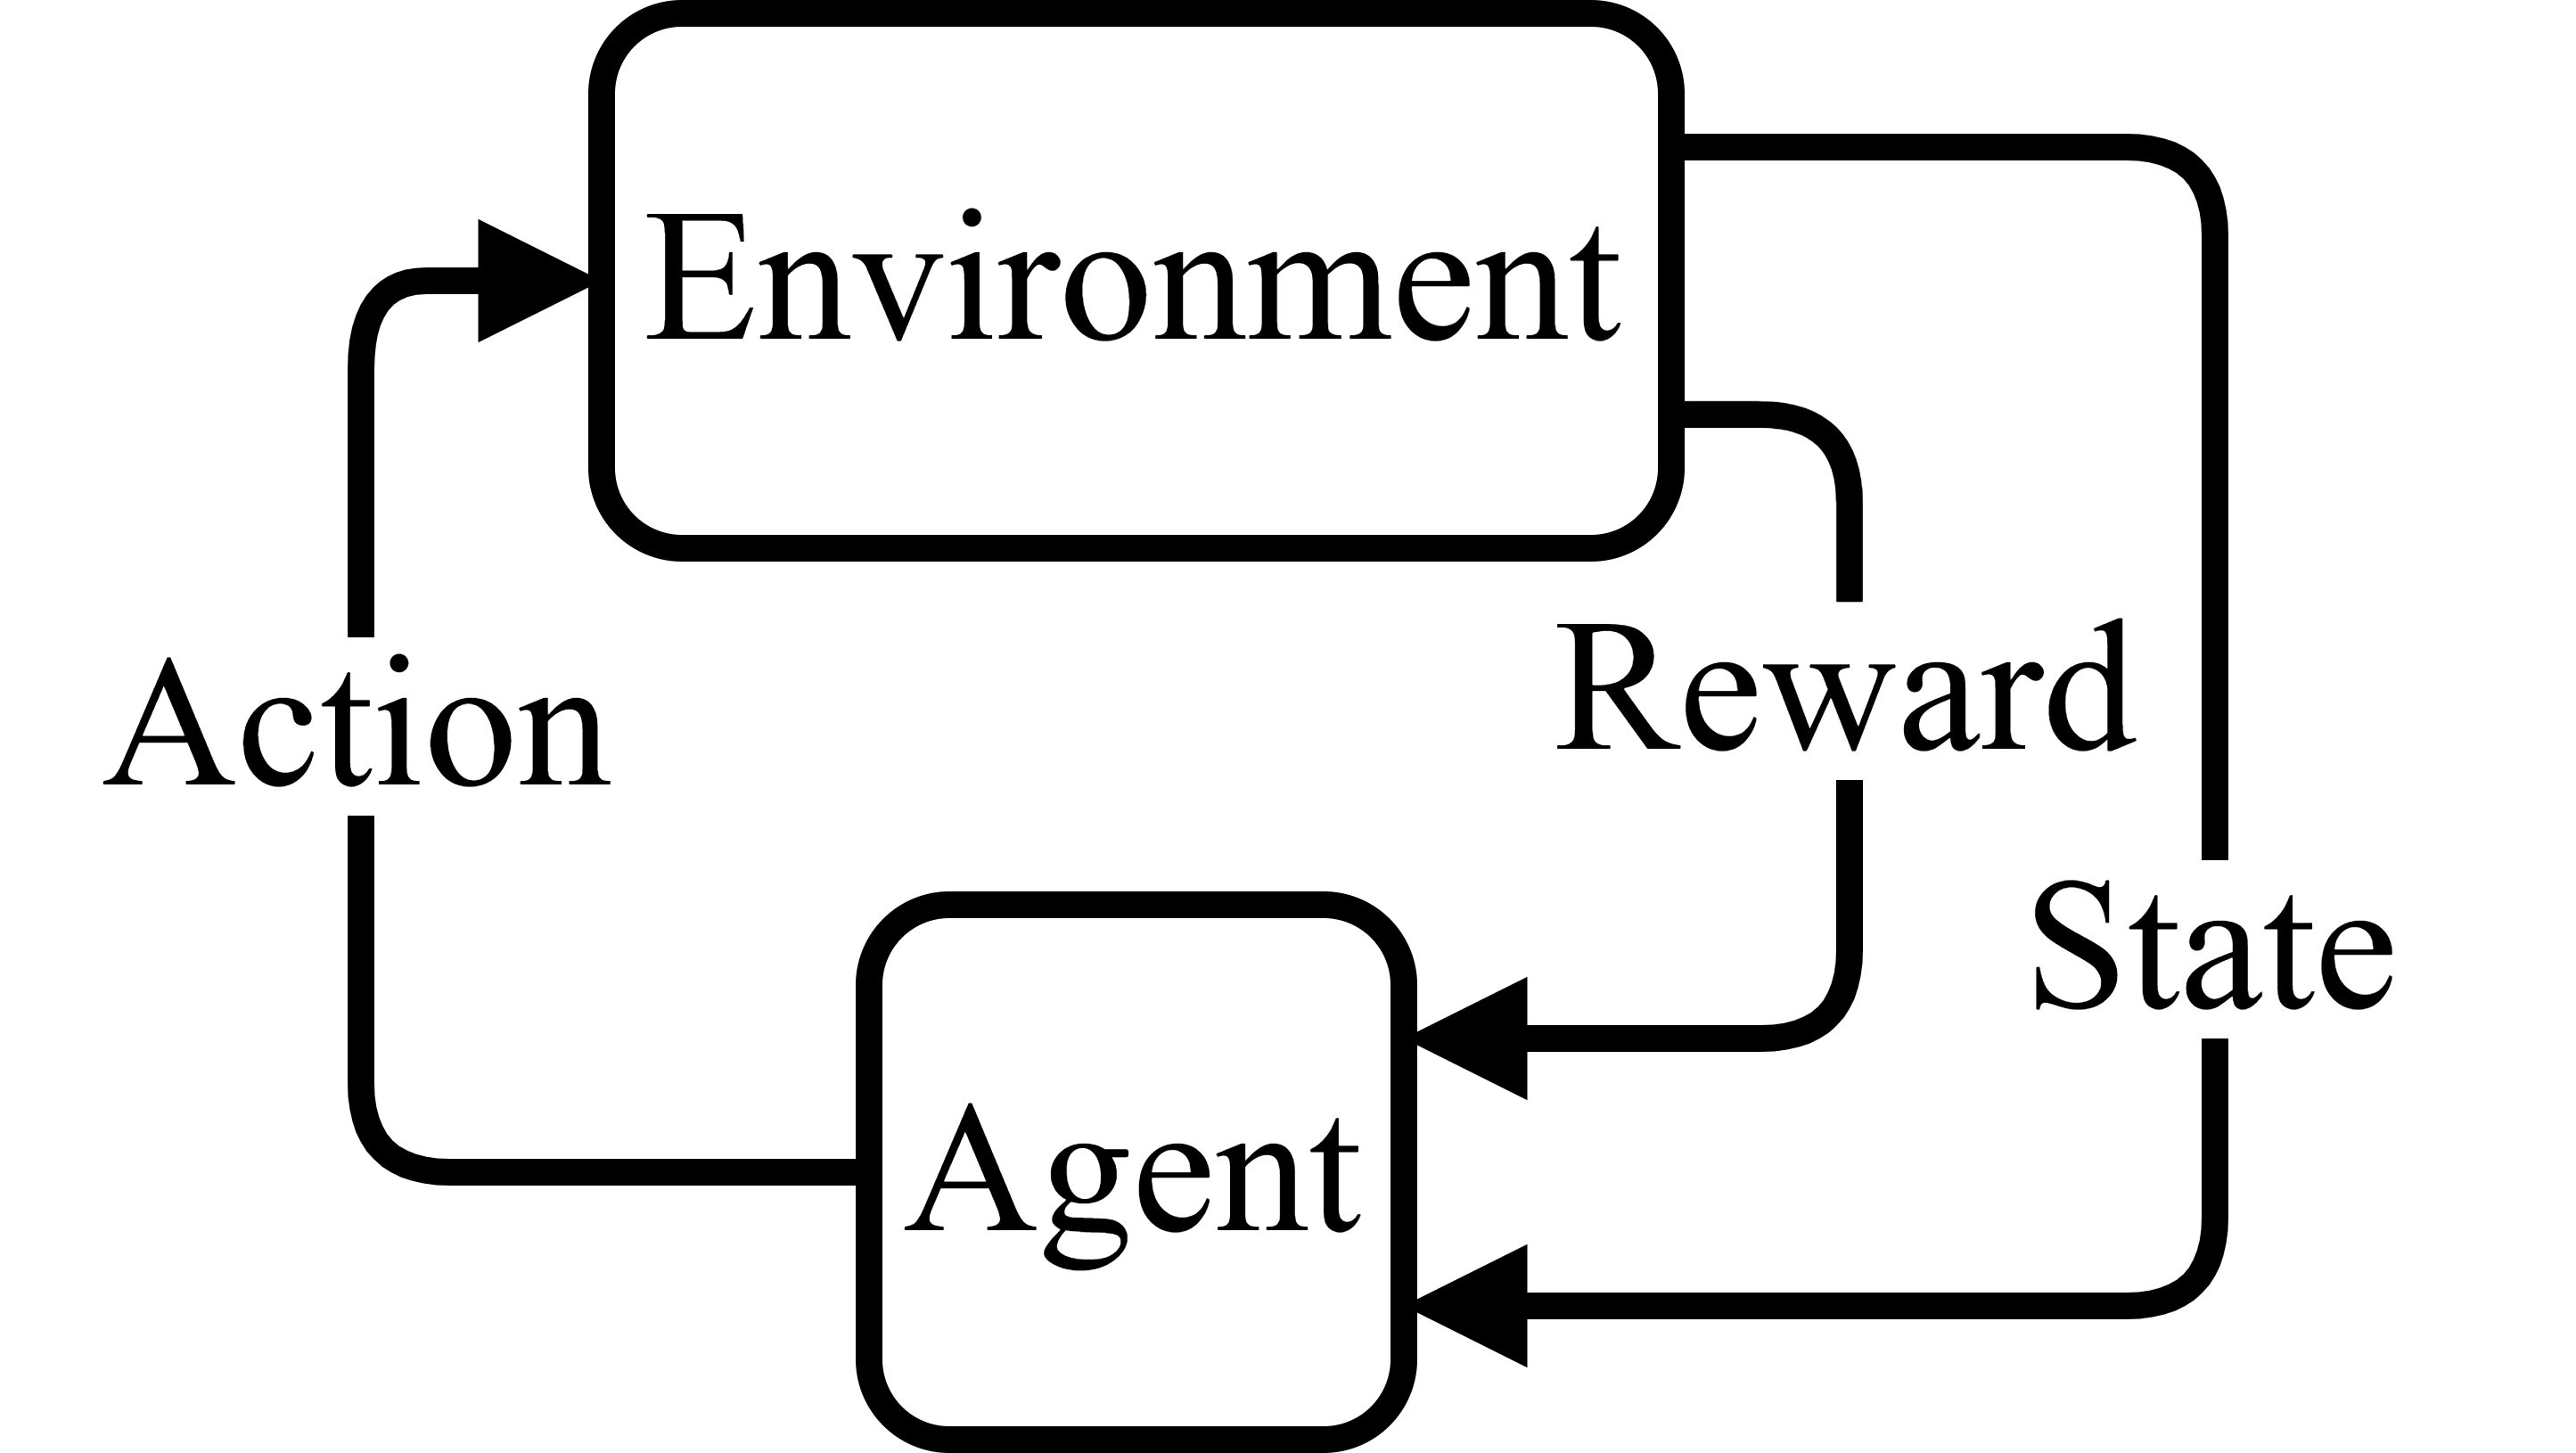
\includegraphics[width=0.55\textwidth]{figures/RL.png}
        \caption{RL Block Diagram}
        \vspace{-0.35 in}
        \label{fig:RL Block Diagram}
    \end{center}
\end{wrapfigure}
%

A solution to combat the nonlinear difficulties is the use of Reinforcement Learning (RL), which takes advantage of neural networks to represent the nonlinear aspects of the control architecture. The RL approach does not require closed-form models of the system dynamics to develop a controller. Rather, the approach creates a machine-learning-based agent to interact with an environment collecting samples of rewards and actions that get mapped to system states, as shown in Figure 3. With this map, the agent defines inputs for the system based in its state. Previous work has shown that this method can be successful at defining both mechanical parameters and control strategies for rigid systems \cite{Ha2019}.
\end{block}

%----------------------------------------------------------------------------------------

\end{column} % End of the first column

% ----------------------------------------------------------------------------------------
\begin{column}{\sepwid}\end{column} % Empty spacer column

% ----------------------------------------------------------------------------------------

% ----- Column Two & Three ---------------------------------------------------------------
\begin{column}{\twocolwid} % Begin a column which is two columns wide (column 2)


%----------------------------------------------------------------------------------------
%	IMPORTANT RESULT
%----------------------------------------------------------------------------------------

\begin{block}{Reinforcement Learning for Flexible Robotics}
%
\begin{wrapfigure}{r}{0.2\textwidth}
    \captionsetup{justification=centering, labelformat=simple}
    \begin{center}
        \vspace{-0.25 in}
        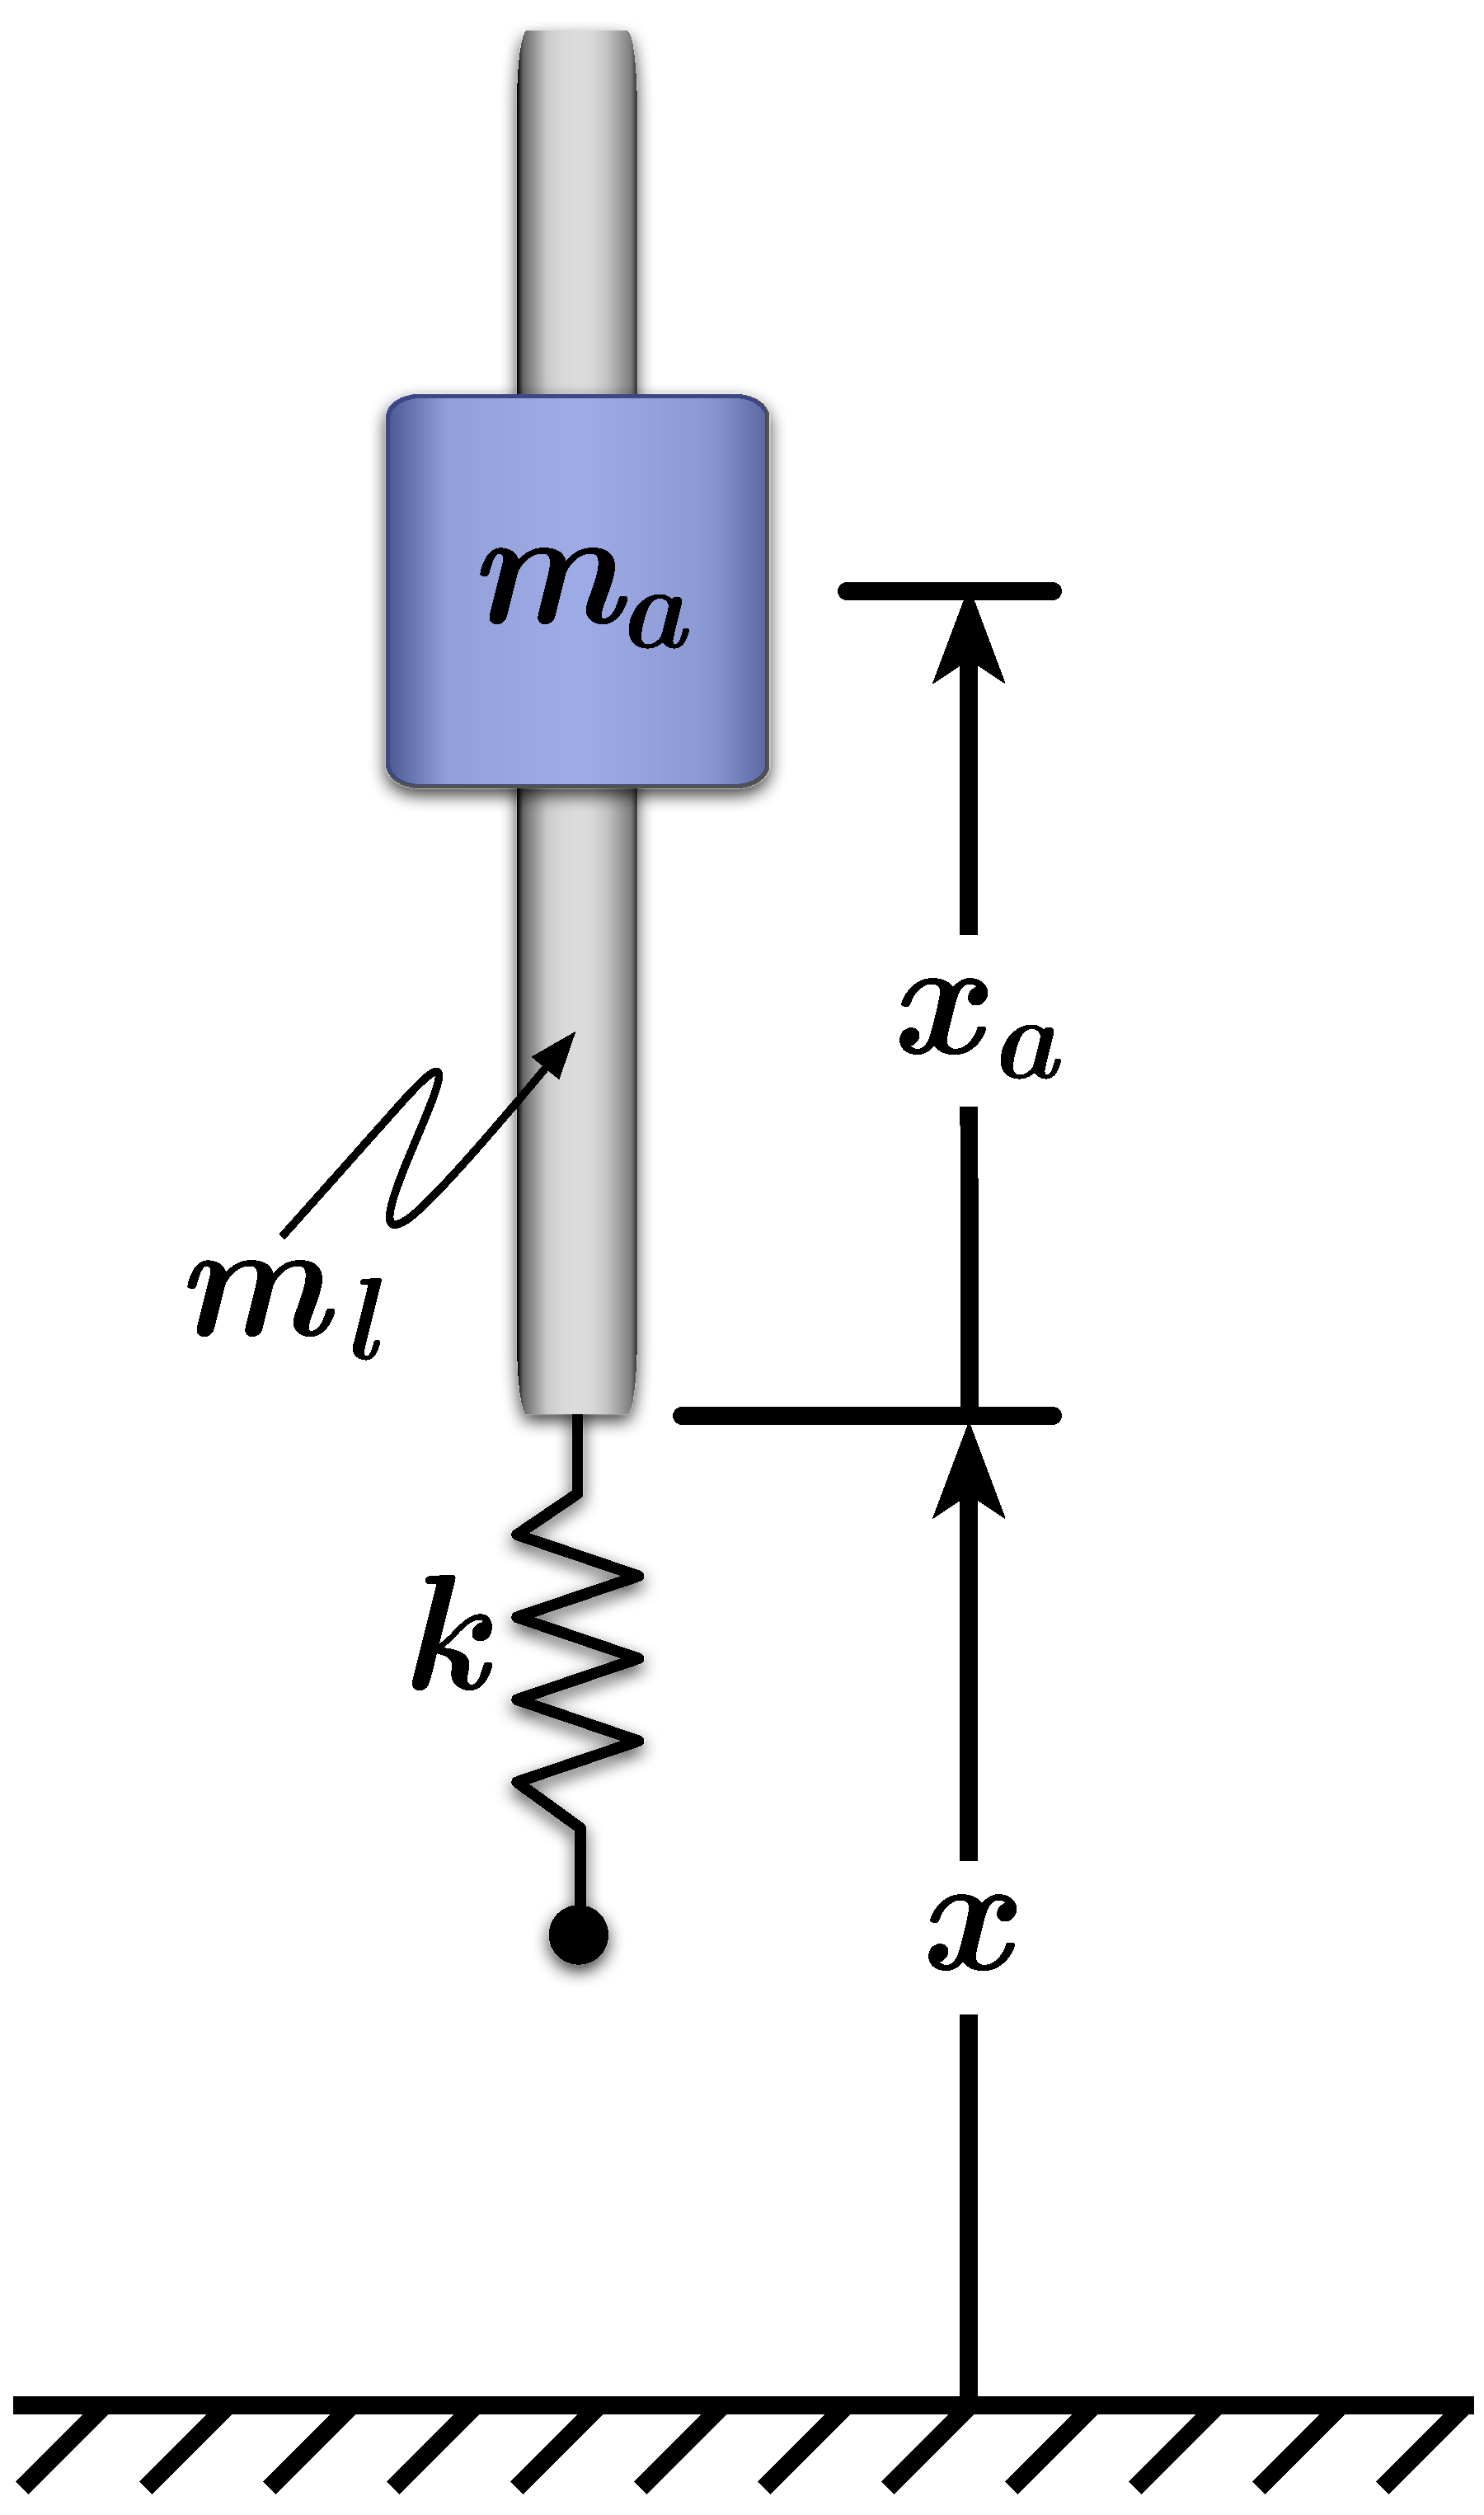
\includegraphics[width=0.17\textwidth]{figures/pogo_stick_model.pdf}
        \caption{Model}
        \vspace{-0.35 in}
        \label{fig:Pogostick}
    \end{center}
\end{wrapfigure}
%

In this work, Reinforcement Learning is used to develop control strategies leading to higher performance, both in desired movement and energy efficiency, for a flexible system. The pogo stick model shown in Figure 4 is used to train an agent to determine the acceleration of the mass, $m_a$, along the rod, $m_l$, causing the system to jump. The agent is tasked with learning a control strategy that jumps as high as possible in a single jump while also limiting power consumption. Two training strategies are deployed to accomplish this task. In the first strategy, the agent is rewarded based on the height it achieves, receiving a score directly proportional to jump height. For the second strategy, the agent is rewarded using a normalized positive score proportional to jump height, and punished a normalized negative score proportional to power use. The agent is able to learn both optimal jumping height strategies and power conserving strategies.
\end{block} 

\begin{columns}[t,totalwidth=\twocolwid] % Split up the two columns wide column

\begin{column}{\onecolwid}\vspace{-.57in} % The first column within column 2 (column 2.1)



% ----- Column Two ----------------------------------------------------------------------

%----------------------------------------------------------------------------------------
%	MATERIALS
%----------------------------------------------------------------------------------------

\begin{block}{Defining The Reward}

    Two reward functions are defined for training the two different agents; the first rewards the agent based on the height it reaches; the second seeks to balance reward height with power usage. The reward function for the second case is: 
    \vspace{0.32in}
    \begin{equation}
        R=\frac{\omega_x\, \frac{x_t - x_{min}}{x_{max} - x_{min}} + m_a\,\omega_p\, \frac{a_t v_t - a_{max} v_{max}}{a_{min} v_{min} - a_{max} v_{max}} - \omega_p}{\omega_x + \omega_p}
        \label{eq:Reward function}
    \end{equation}
    \vspace{-0.18in}

    where $x_t$, $a_t$ and $v_t$ are position, velocity and acceleration of mass $m_a$, respectively, and $\omega_{x}$ and $\omega_{p}$ are weights used to tune the relative contributions of jump height and power use. 
\end{block}

%----------------------------------------------------------------------------------------
\begin{block}{Jumping Analysis}
% max heights are 0.286 and 0.161
The jumping height data presented in Figure 5 shows that when training the agent to jump high regardless of power usage, the maximum jump height reached is higher than when training the agent to conserve power. The maximum height reached by the power conserving agent is 56\% of the height reached by the agent trained to only jump high. However, the power consumption data in Figure 6 shows that the power conserving agent is more energy efficient, using 64\% less power. Comparing the maximum jump height reached to the power used to get there, the the power conserving agent has learned a more efficient control strategy.
\end{block}

%----------------------------------------------------------------------------------------

\end{column} % End of column 2.1


% ----- Column Three --------------------------------------------------------------------
\begin{column}{\onecolwid}\vspace{-.57in} % The second column within column 2 (column 2.2)

%----------------------------------------------------------------------------------------
%	METHODS
%----------------------------------------------------------------------------------------

\begin{block}{Evaluation Data}
%
    \begin{figure}[tb]
        \captionsetup{justification=centering, labelformat=simple}
        \vspace{0.5in}
                \begin{center}
                    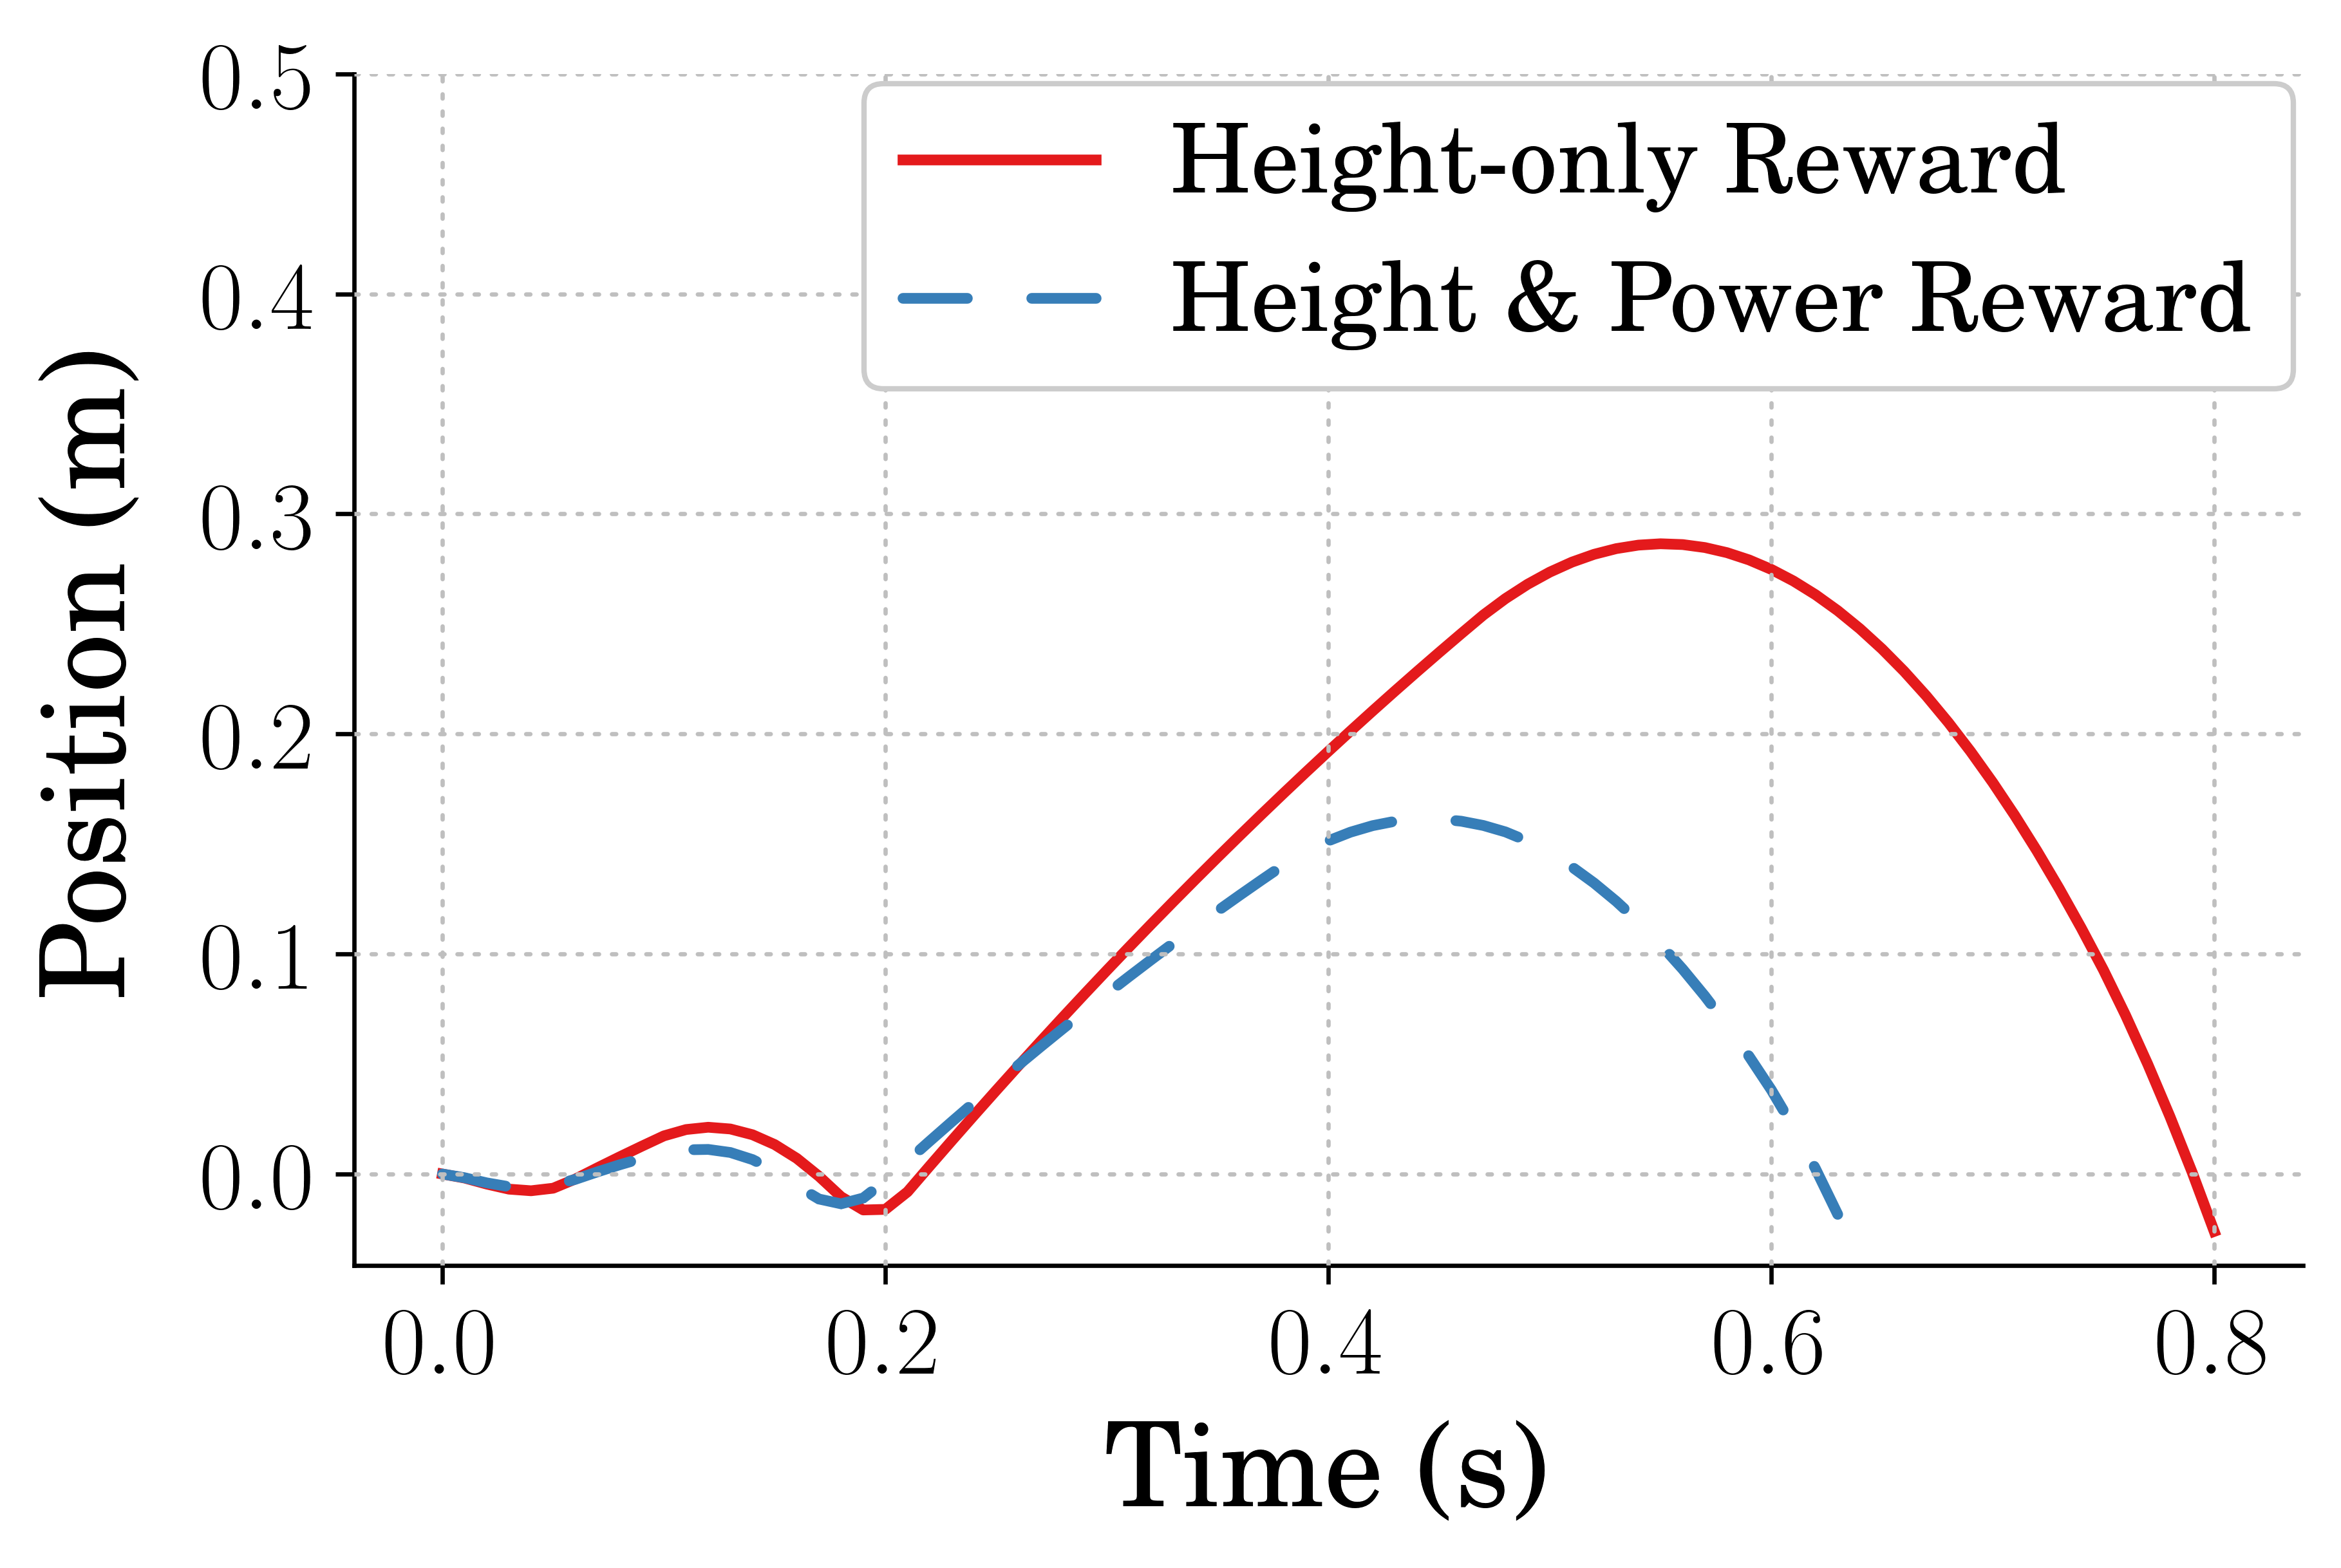
\includegraphics[width = \columnwidth]{figures/PosVsTime_2021-03-22_133925.png}
                    \caption{\:Jumping Height Comparison}
                    \label{fig:Jumping Height Comparison}
                \end{center}
        \vspace{-0.2in}
    \end{figure}
    %
    \begin{figure}[tb]
        \captionsetup{justification=centering, labelformat=simple}
        \vspace{0.5in}
                \begin{center}
                    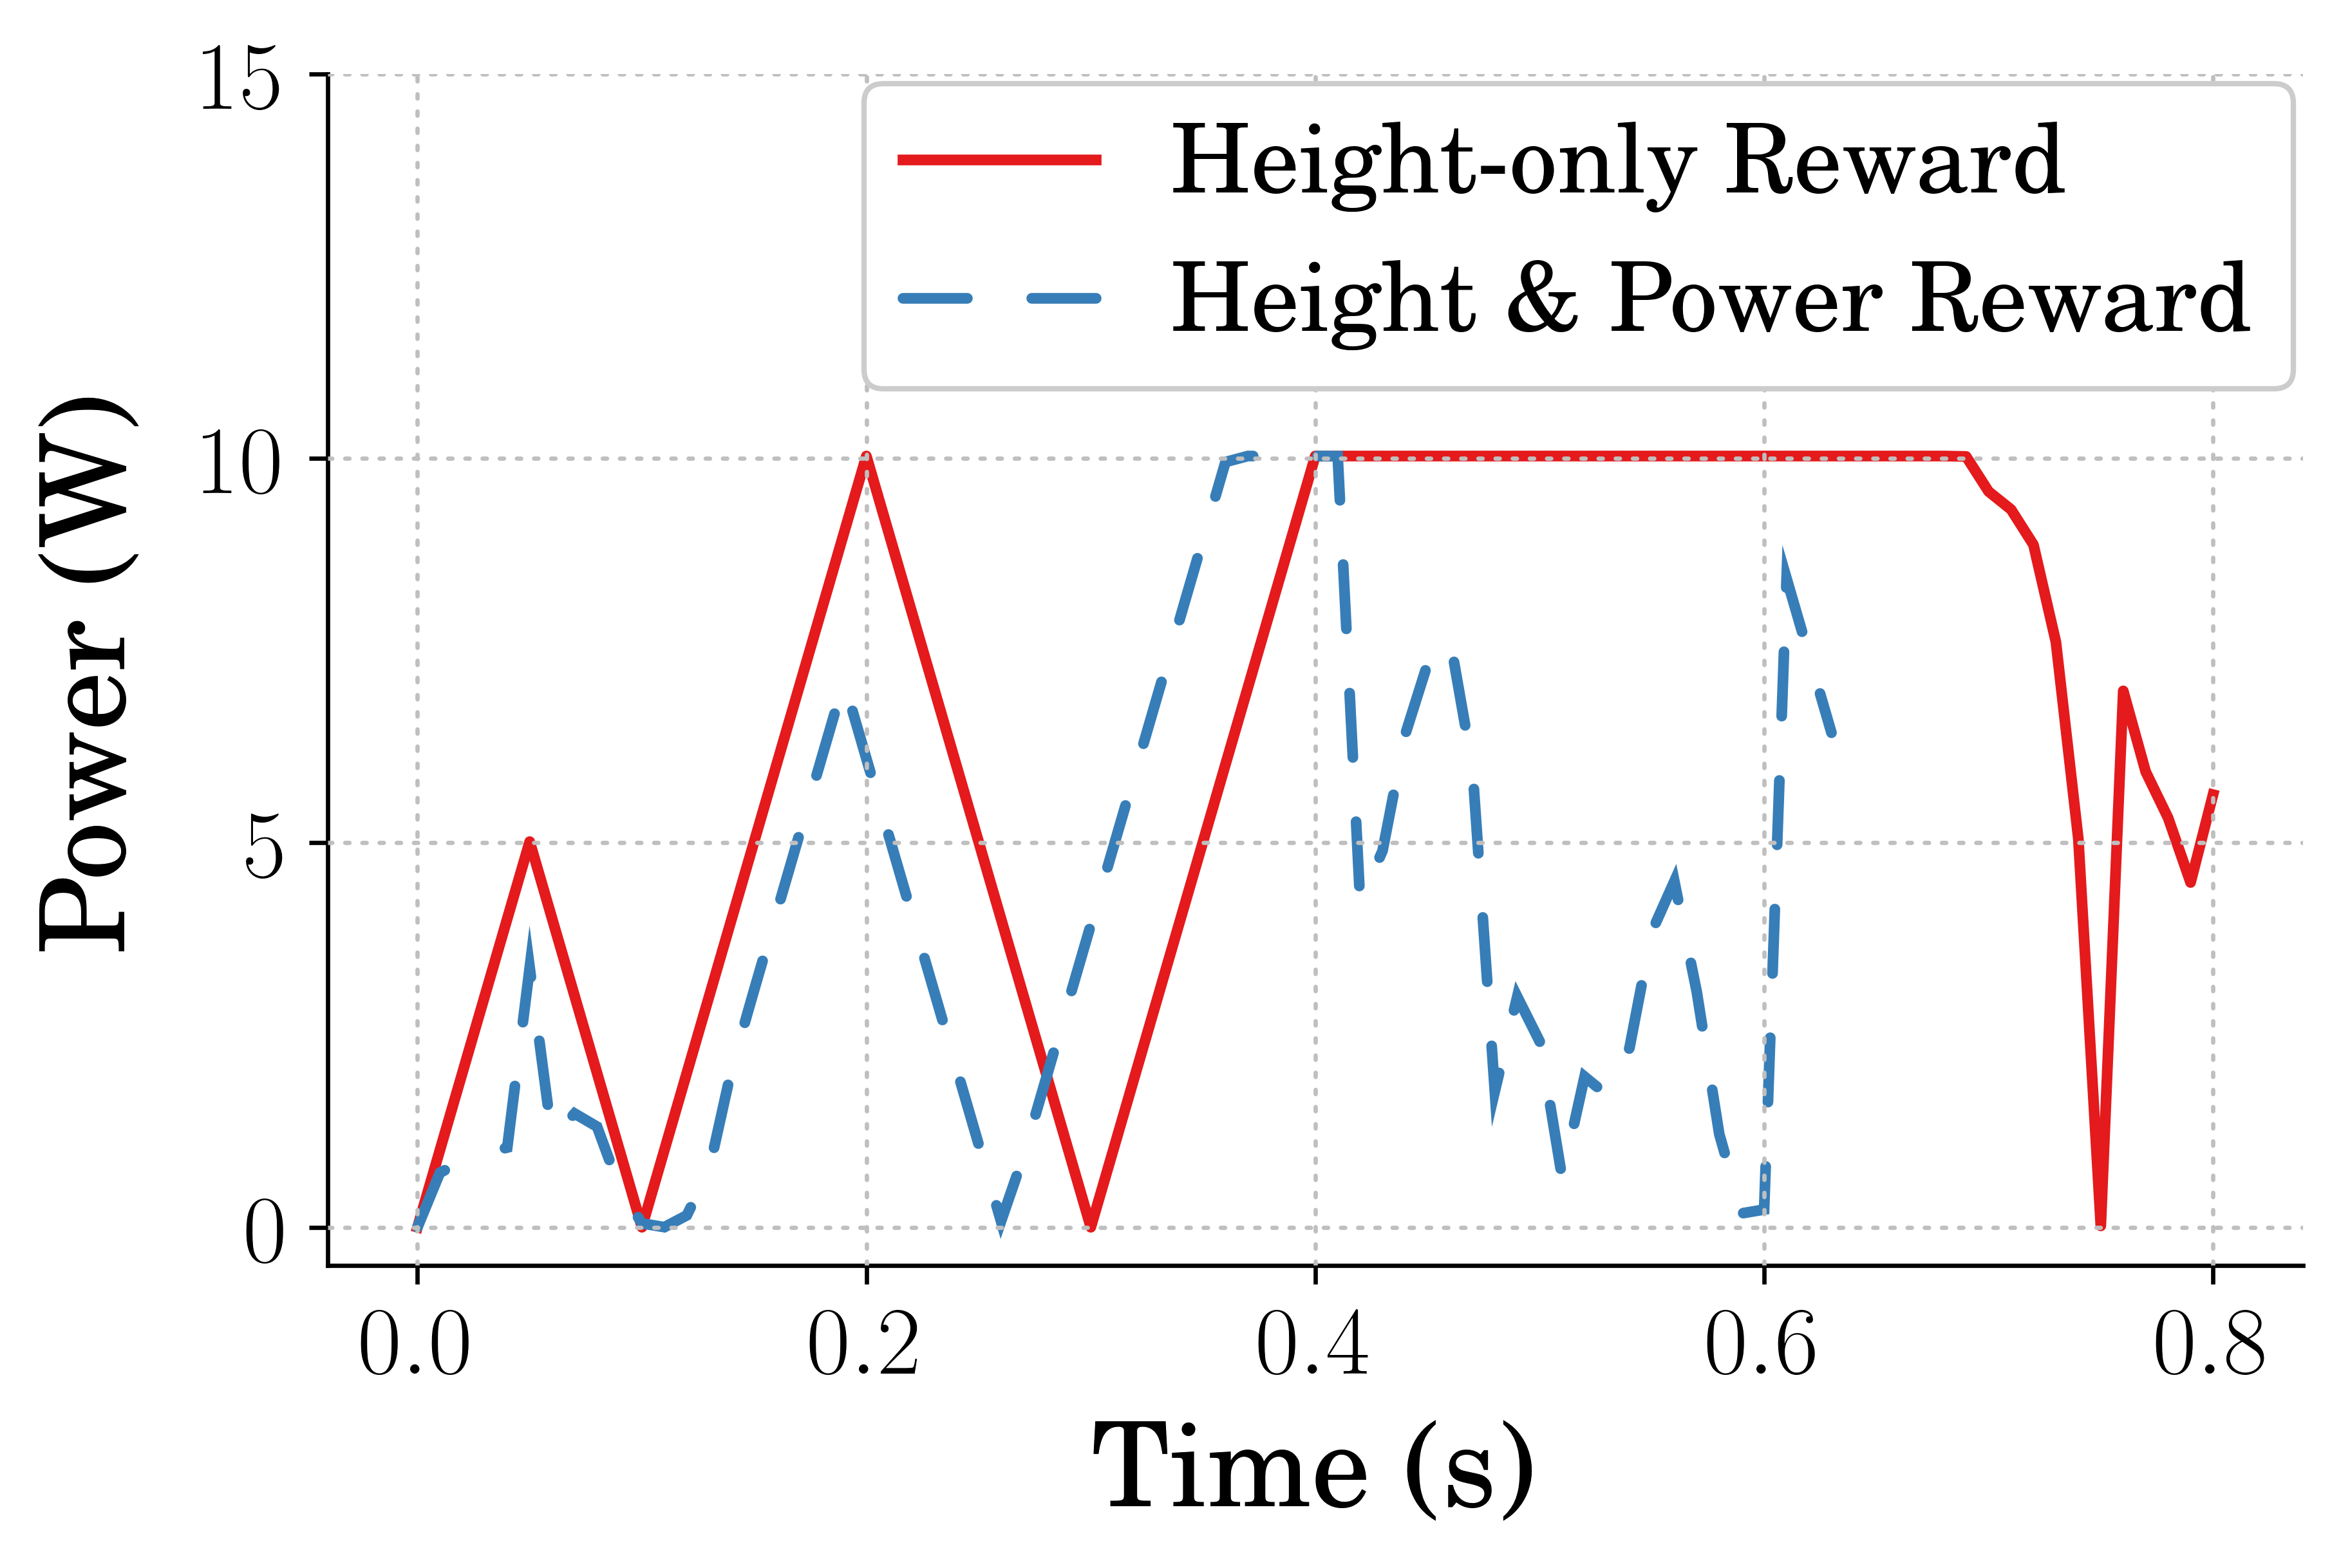
\includegraphics[width = \columnwidth]{figures/PowVsTime_2021-03-22_133929.png}
                    \caption{\:Power Usage Comparison}
                    \label{fig:Power Usage Comparison}
                \end{center}
        \vspace{-0.2in}
    \end{figure}
    %

\end{block}

%----------------------------------------------------------------------------------------

\end{column} % End of column 2.2

\end{columns} % End of the split of column 2 - any content after this will now take up 2 columns width

%----------------------------------------------------------------------------------------

\begin{columns}[t,totalwidth=\twocolwid] % Split up the two columns wide column again

\begin{column}{\onecolwid} % The first column within column 2 (column 2.1)

%----------------------------------------------------------------------------------------
%	MATHEMATICAL SECTION
%----------------------------------------------------------------------------------------
% \begin{block}{Defining The Reward}
%     \vspace{-8.75in}

%     For this work, two reward functions were defined for training two different agents. The first rewards the agent based on the height it reaches. The second seeks to balance reward height with power usage. The reward function used can be expressed as an equation 
%     \vspace{-.1in}
%     \begin{equation}
%         R=\frac{\frac{x_t - x_{min}}{x_{max} - x_{min}}\, \omega_x + m_a\, \frac{a_t v_t - a_{max} v_{max}}{a_{min} v_{min} - a_{max} v_{max}}\, \omega_p - \omega_p}{\omega_x + \omega_p}
%         \label{eq:Reward function}
%     \end{equation}
%     \vspace{0.1in}

%     where $x_t$, $a_t$ and $v_t$ are position, velocity and acceleration of mass $m_a$ respectively, \omega_x and \omega_p are weights used to tune how much 
% \end{block}

%----------------------------------------------------------------------------------------

\end{column} % End of column 2.1

\begin{column}{\onecolwid} % The second column within column 2 (column 2.2)

%----------------------------------------------------------------------------------------
%	RESULTS
%----------------------------------------------------------------------------------------
% \begin{block}{Defining the Reward}
% %
% Using the weights $\omega_x$ and $\omega_p$, the reward function (1) can be tuned to guide the agents learning process towards maximizing power efficiency. 

% \begin{equation}
%     R=\frac{\frac{x_t - x_{min}}{x_{max} - x_{min}}\, \omega_x + m_a\, \frac{a_t v_t - a_{min} v_{min}}{a_{max} v_{max} - a_{min} v_{min}}\, \omega_p - \omega_p}{\omega_x - \omega_p}
%     \label{eq:Reward function}
% \end{equation}
% \vspace{0.2in}

% where $x_t$, $a_t$ and $v_t$ are position, velocity and acceleration respectively.

% \end{block}

%----------------------------------------------------------------------------------------

\end{column} % End of column 2.2

\end{columns} % End of the split of column 2

\end{column} % End of the second column

\begin{column}{\sepwid}\end{column} % Empty spacer column



\begin{column}{\onecolwid} % The third column

%----------------------------------------------------------------------------------------
%	IMPLICATION OF RESULTS
%----------------------------------------------------------------------------------------

\begin{block}{Implications of Results}
%
\begin{wrapfigure}{r}{0.5\textwidth}
    \captionsetup{justification=centering, labelformat=simple}
    \begin{center}
        \vspace{-0.25 in}
        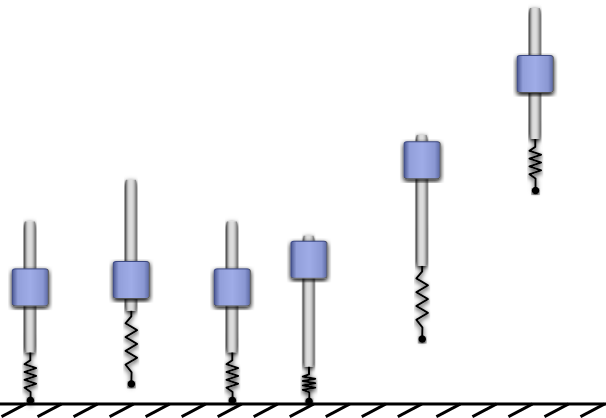
\includegraphics[width=0.46\textwidth]{figures/stutter_jump.png}
        \caption{Stutter Jump \cite{Vaughan2013}}
        \label{Stutter Jump}
        \vspace{-0.5 in}
    \end{center}
\end{wrapfigure}
%
The jumping profiles presented in Figure 5 show that the agent is controlling the pogo stick to jump with a profile matching a stutter jump profile, which can be seen in Figure 7. This kind of jump is optimal for reaching maximum heights \cite{Vaughan2013}. The reinforcement learning agent learned optimal jumping strategies while minimizing power consumption for the simple model of a flexible legged locomotion system.
\end{block}

%----------------------------------------------------------------------------------------
%	ADDITIONAL INFORMATION
%----------------------------------------------------------------------------------------

% \begin{block}{Additional Information}

% Maecenas ultricies feugiat velit non mattis. Fusce tempus arcu id ligula varius dictum. 
% \begin{itemize}
% \item Curabitur pellentesque dignissim
% \item Eu facilisis est tempus quis
% \item Duis porta consequat lorem
% \end{itemize}

% \end{block}

%----------------------------------------------------------------------------------------
%	CONCLUSION
%----------------------------------------------------------------------------------------

\begin{block}{Conclusion}

Using a reinforcement learning approach to define control strategies for flexible jumping systems leads to optimal performance. Using a correctly tuned reward function can further improve performance, leading to control strategies that require less power. 

\end{block}




%----------------------------------------------------------------------------------------
%	REFERENCES
%----------------------------------------------------------------------------------------
\begin{block}{References}

%\nocite{*} % Insert publications even if they are not cited in the poster
\small{\bibliographystyle{unsrt}
\bibliography{CRAWLAB-Writing-IMECE-2021.bib}}

\end{block}





%----------------------------------------------------------------------------------------
%	ACKNOWLEDGEMENTS
%----------------------------------------------------------------------------------------
\begin{block}{Acknowledgements}

\small{\rmfamily{Special thanks to the Louisiana Crawfish Promotion and Research Board for their support.}} \\

\end{block}



\end{column} % End of the third column

\end{columns} % End of all the columns in the poster

\end{frame} % End of the enclosing frame

\end{document}
